\section{Making COVID-19 time series interactive}

The main feature the user interacts with in our application is the chart analysis page as shown in figure \ref{fig:screenshot-chart}. The goal was to provide a powerful tool that can still be managed by an average user.


\subsection{User Features}
The user is able to select countries, and within countries show features such as cases, fatalities, tests, test positivity rate, and vaccinations. The different time series are automatically assigned a different color in case of countries or a different line dash pattern in case of features. Additionally, the user can choose the color they want to use for which country. For example, they might want to use red for Switzerland and blue for France. The different time series can be hidden or shown, without having to be removed.

The center chart shows the selected data and provides detailed information on hover. It displays the value of each series in a tooltip. We used d3.js to build this visualization.

The user can further change between absolute (totals) or daily rates. Should they decide to visualize absolute data, they might want to change the scale from linear to a log scale.

Furthermore, they can add a rolling mean or rolling sum with a given window size. To compare between countries, it is helpful to activate normalization by population. The user can choose between several population factors.

The visualizations also instantly update upon change of a setting. This is because the frontend makes exactly one call per country to the backend and retrieves the data for all features in the given time frame. This usually takes less than 200ms (measured by the client, which includes network latency)). From that point on, the frontend application computes all the transformations in the browser.

\subsection{Use Case Example}
A user might live in Switzerland. Switzerland has defined that if a country has 60 more cases in the last 14 days per 100,000 inhabitants than Switzerland, they will put it on the list of risk countries\footnote{\href{https://www.bag.admin.ch/bag/en/home/krankheiten/ausbrueche-epidemien-pandemien/aktuelle-ausbrueche-epidemien/novel-cov/empfehlungen-fuer-reisende/quarantaene-einreisende.html}{https://www.bag.admin.ch/bag/en/home/krankheiten/ausbrueche-epidemien-pandemien/aktuelle-ausbrueche-epidemien/novel-cov/empfehlungen-fuer-reisende/quarantaene-einreisende.html}}. 
To figure out if a given country should be on the list or vice versa, a user would go through the following steps in our application to create the visualization that gives them an answer:

\begin{itemize}
    \item Add Switzerland and another country to the chart. Select cases.
    \item Select daily data (default)
    \item Select rolling sum of 14 days
    \item Optionally select smoothing of 7 days to make the chart easier to read (this introduces a slight imperfection in the data)
    \item Select By Population of 100,000
    \item Select a shorter time frame to focus in on the recent weeks
\end{itemize}

The resulting chart can be seen in figure \ref{fig:che-vs-nld}.

\begin{figure}
\centerline{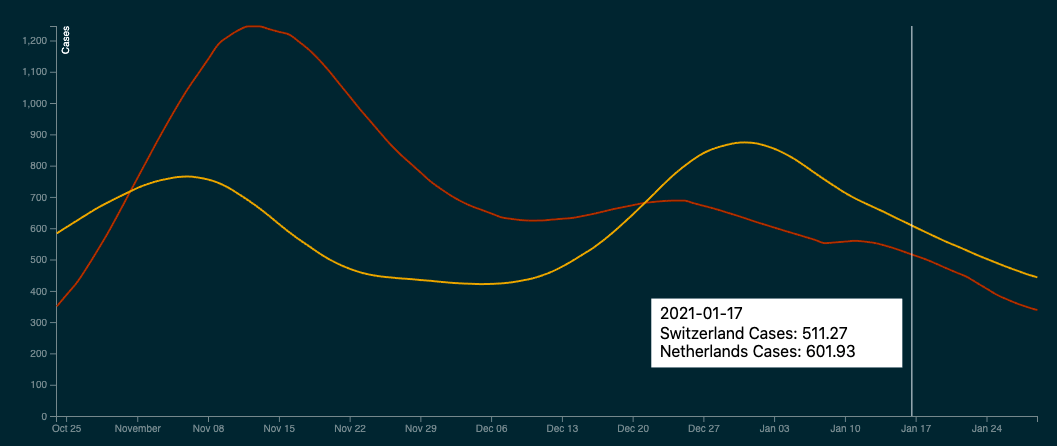
\includegraphics[scale=.23]{figs/che-vs-nld.png}}
\caption{The chart shows that the Netherlands has an incidence rate 90.66 higher than Switzerland on January 17, 2021. This should mean the Netherlands should be on the list of risk countries of Switzerland. It was not at the time of writing, which shows the government applies some leniency in their rules. It is probably not on the list because the trend is similar to the one of Switzerland and showing good signs. They also use an arbitrary cut-off date. A user interpreting this graph is able to read this information from it and can make their own conclusions which shows  the potency of our solution.}
\label{fig:che-vs-nld}
\end{figure}
